%
% $RCSfile: double_hierarchy.tex,v $
%
% Copyright (c) 2005-2006. Christian Heller. All rights reserved.
%
% Permission is granted to copy, distribute and/or modify this document
% under the terms of the GNU Free Documentation License, Version 1.1 or
% any later version published by the Free Software Foundation; with no
% Invariant Sections, with no Front-Cover Texts and with no Back-Cover
% Texts. A copy of the license is included in the section entitled
% "GNU Free Documentation License".
%
% http://www.cybop.net
% - Cybernetics Oriented Programming -
%
% http://www.resmedicinae.org
% - Information in Medicine -
%
% Version: $Revision: 1.1 $ $Date: 2006-01-03 08:21:45 $ $Author: christian $
% Authors: Christian Heller <christian.heller@tuxtax.de>
%

\subsubsection{Double Hierarchy}
\label{double_hierarchy_heading}

Finally, what makes up the character of a model (in the understanding of the
human mind) is a combination of two hierarchies: the \emph{Parts} it consists
of, together with \emph{Meta Information} about it.

Most properties of a molecule in \emph{Chemistry}, for example, are determined
by the number and arrangement of its atoms. \emph{Hydrogen} (H$_{2}$) becomes
\emph{Water} (H$_{2}$O) (with a totally different character) when just one
\emph{Oxygen} (O) atom is added per hydrogen molecule.

The kinds of meta information discussed in \cite{heller2004} were also called
\emph{Dimensions} or \emph{Conceptual Interaction} between a \emph{Whole} and
its \emph{Parts}. They may represent very different properties and be
constrained to certain\\values- or areas of validity.

\begin{figure}[ht]
    \begin{center}
        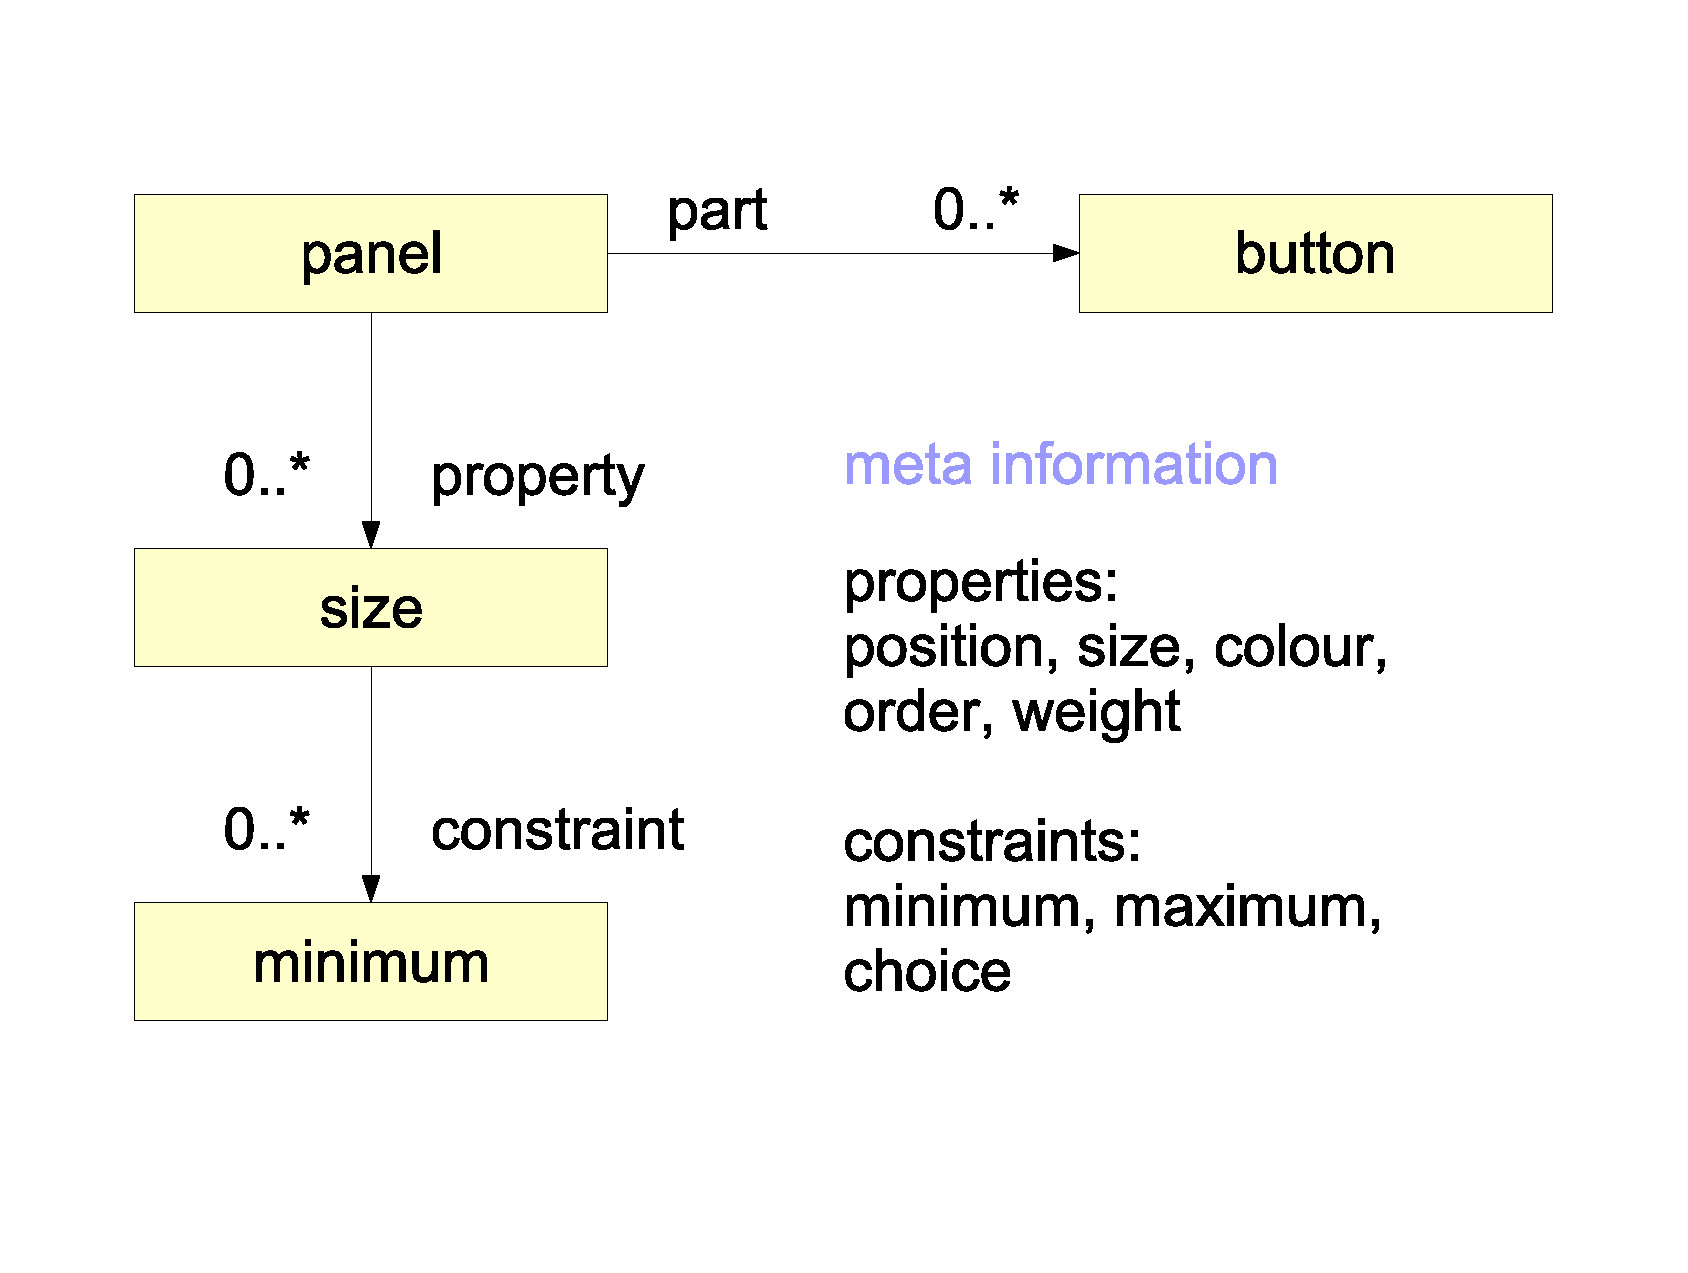
\includegraphics[scale=0.2]{vector/double.eps}
        \caption{Double Hierarchy (Parts $\vert$ Meta Info)}
        \label{double_figure}
    \end{center}
\end{figure}

Figure \ref{double_figure} illustrates the \emph{Double Hierarchy}\\here
spoken of. A graphical panel was chosen as example model. It consists of
smaller parts, among them being a number of buttons. Altogether they form the
\emph{Part Hierarchy}. On the other hand, there are properties like the size,
position or colour of the buttons, which are neither part of the panel, nor of
the buttons themselves; they are information \emph{about} the buttons and form
an own \emph{Meta Hierarchy}. To the latter do also belong constraints like the
minimum size of a button or a possible choice of colours for it.
\emph{Properties} are (meta) information about a \emph{Part};
\emph{Constraints} about a \emph{Property}.
